% vim:encoding=utf8 ft=tex sts=2 sw=2 et:

\documentclass{classrep}
\usepackage[utf8]{inputenc}
\usepackage{color}
\usepackage{mathtools}

\usepackage{subfig}
\usepackage{float}

\usepackage[labelfont=it]{caption}

\studycycle{Informatyka, studia niestacjonarne, mgr II st.}
\coursesemester{I}

\coursename{Przetwarzanie obrazu i dźwięku}
\courseyear{2015/2016}

\courseteacher{mgr inż. Piotr Ożdżyński}
\coursegroup{Sobota, 14:15}

\author{
  \studentinfo{Jakub Antosik}{206788} \and
  \studentinfo{Andrzej Lisowski}{206807} 
}

\title{Zadanie 2: Filtracja w dziedzinie częstotliwości i segmentacja obrazu.}

\begin{document}
\maketitle

\section{Cel}
Celem zadania było zapoznanie się z transformatą Fouriera, filtracją w dziedzinie częstotliwości oraz segmentacją obrazu. W części implementacyjnej należało stworzyć program w wybranym przez siebie języku programowania, który będzie w stanie przeprowadzić analizowane operacje. Do tego celu wykorzystano aplikację z zadania 1.\\
\\
\indent
Szczegółowy opis zadania został przedstawiony w [1].

\section{Wprowadzenie}
Filtracje obrazów można podzielić na realizowane w układzie przestrzennym i w dziedzinie częstotliwości. Pierwsze zagadnienie było analizowane w zadaniu 1. Poniższe sprawozdanie przedstawia badanie drugiej grupy filtracji - przeprowadzanych w dziedzinie częstotliwości.  

\subsection{Transformata Fouriera i odwrotna transformata Fouriera}
Transformata Fouriera umożliwia przekształcenie obrazu z układu przestrzennego w reprezentację częstotliwościową. Znajduje ona zastosowanie w fitracji próbki, co jest spowodowane bardzo łatwą modyfikacją wybranych grup częstotliwości. DFT jest operacją całkowicie odwracalną, więc po nałożeniu filtru wykorzystuje się transformatę odwrotną i otrzymuje zmodyfikowany obraz. Dokładny opis DFT i IDFT znajduje się w [2].

\subsection{Szybka transformata Fouriera i odwrotna szybka transformata Fouriera}
Dyskretna transformata Fouriera jest operacją o złożoności obliczeniowej $\mathcal{O}(N^{2})$. Pojawiło się kilka propozycji umożliwiających optymalizację tego procesu. Jedną z nich jest jest algorytm Cooleya-Tukeya o złożoności $\mathcal{O}(N\log{2}N)$, bazujący na metodzie dziel i zwyciężaj. Dokładny opis FFT i IFFT znajduje się w [11].

\subsection{Filtracja}
Jednym z zastosowań transformaty Fouriera jest możliwość szybkiej filtracji obrazów. W poniższej sekcji przedstawione zostały przeanalizowane metody.

\subsubsection{Filtr dolnoprzepustowy (górnozaporowy)}
Filtr dolnoprzepustowy jest używany do usuwania pikseli o wysokiej częstotliwości. Jako parametr przyjmuje maksymalną wartość piksela (częstotliwości), który znajdzie się w zmodyfikowanym obrazie. Jest on wykorzystywany do usuwania szumów.

\subsubsection{Filtr górnoprzepustowy (dolnozaporowy)}
Filtr górnoprzepustowy jest używany do usuwania pikseli o niskiej częstotliwości. Jako parametr przyjmuje minimalną wartość piksela (częstotliwości), który znajdzie się w zmodyfikowanym obrazie. Jest on wykorzystywany do wyostrzania krawędzi.

\subsubsection{Filtr pasmowoprzepustowy}
Filtr górnoprzepustowy jest używany do usuwania pikseli o niskich i wysokich częstotliwościach. Jako parametry przyjmuje minimalną i maksymalną wartość pikseli (częstotliwości), które znajdą się w zmodyfikowanym obrazie.

\subsubsection{Filtr pasmowozaporowy}
Filtr pasmowozaporowy jest używany do usuwania pikseli o częstotliwościach środkowych. Jako parametry przyjmuje minimalną i maksymalną wartość pikseli (częstotliwości), które zostaną usunięte z modyfikowanego obrazu.

\subsubsection{Filtr z detekcją krawędzi}
Filtr z detekcją krawędzi jest modyfikacją filtru górnoprzepustowego. Jest używany do usuwania pikseli o niskiej częstotliwości. Jako parametry przyjmuje minimalną wartość piksela (częstotliwości), który znajdzie się w zmodyfikowanym obrazie oraz maskę. Jest on wykorzystywany do wyostrzania krawędzi położnych w konkretnym kierunku (np. N-S, E-W).

\subsubsection{Filtr modyfikujący fazę widma transformaty Fouriera}
Filtr modyfikujący fazę widma transformaty Foueriera jest wykorzystywany do podzielenia obrazu na 4 części o wybranych rozmiarach. Jako parametry przyjmuje stałe całkowite \textit{k} i \textit{l} będące współczynnikami przesunięcia obrazu.

\subsection{Okno Hanninga}
Okna czasowe są wykorzystywane do poprawy charakterystyki próbkowanego sygnału. Transformata Fouriera przyjmuje, że analizowany sygnał jest sygnałem ciągłym, natomiast w rzeczywistości jest on dyskretny. Powoduje to w rezultacie ścięty przebieg falowy, który ma wpływ na wyciek widma. Jednym z okien czasowych jest okno Hanninga. Polega ono na wymnożeniu piseli obrazu w dziedzieni czasu wg następującego wzoru:\\
\[ w(n) = 0.5 * (1 - cos \frac{2 \ast \pi \ast n}{N - 1}) \]
\\
gdzie:\\
\textit{w(n)} - wartość piksela po nałożeniu okna,\\
\textit{n} - numer piksela w sygnale 1D,\\
\textit{N} - liczba pikseli w sygnale 1D.\\

\subsection{Segmentacja}
Segmentacja obrazu jest procesem podzielenia go na zbiór regionów, będących jednorodnymi pod względem założonych wcześniej parametrów. Poniższa sekcja przedstawia opis dwóch metod segmentacji - rozrostu i podziału obszarów.

\subsubsection{Metoda rozrostu obszarów}
Metoda rozrostu obszarów polega na wyborze określonej liczby pikseli, będących \textit{ziarnami}. Wartość ziarna jest porównywana z sąsiadującymi pikselami. Jeżeli są podobne, tzn. ich miara podobieństwa spełnia wybrane wcześniej kryteria, sąsiad jest dołączany do regionu. Rozrost trwa do momentu aż obszar nie potrafi znaleźć dodatkowych, podobnych do niego pikseli. Następnie kolejne ziarna rozpoczynają tworzenie homogenicznego regionu, aż do wykorzystania wszystkich z nich. 

\subsubsection{Metoda podziału obszarów}
Metoda podziału obszarów składa się z dwóch operacji. Pierwszym krokiem jest rekurencyjny podział próbki na zbiór jednolitych regionów. Miara podobieństwa pikseli jest ustalona wcześniej. Następnie następuje łączenie podobnych obszarów.

\section{Opis implementacji}
Opis implementacji został przedstawiony w sprawozdaniu do zadania 1 [3]. Zadanie 2 zostało zrealizowane poprzez rozszerzenie funkcjonalności programu o dodatkowe metody - transformatę Fouriera, filtracje w dziedzinie częstotliwości oraz segmentację obrazów.\\
\\
\indent
Szybka transformata Fouriera została zrealizowana w oparciu o algorytm Cooleya-Tukeya dla obrazów o liczbie pikseli będącej wielokrotnością liczby 2. Funkcjonalności segmentacji zostały zaimplementowane z wykorzystaniem sterty umożliwiającej rozrost regionów. Do podziału obszarów wykorzystano zmodyfikowane drzewo czwórkowe.

\section{Materiały i metody}
Opis materiałów został przedstawiony w sprawozdaniu do zadania 1 [3]. Poniżej zamieszczono maski użyte w filtrze z detekcją krawędzi.
\begin{figure}[H]%
    \centering
    \subfloat[Maska 1]{{
\includegraphics[width=3cm,height=3cm,keepaspectratio]{img/original/edge-detection/mask/F5mask1.png}}}%
    \qquad
    \qquad
    \subfloat[Maska 2]{{
\includegraphics[width=3cm,height=3cm,keepaspectratio]{img/original/edge-detection/mask/F5mask2.png}}}%
    \caption{Maski użyte w filtrze z detekcją krawędzi.}%
\end{figure} 

\section{Wyniki}
Sekcja prezentuje wyniki przeprowadzanej analizy filtracji w dziedzinie częstotliwości oraz segmentacji obrazów.

\subsection{Szybka transformata Fouriera i odwrotna szybka transformata Fouriera}
Poniżej przedstawione zostały widma mocy i widma fazy dla wybranych obrazów 8- i 24-bitowych.

\begin{figure}[H]%
    \centering
    \subfloat[Widmo mocy]{{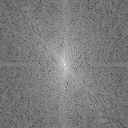
\includegraphics[width=3cm,height=3cm,keepaspectratio]{img/transformed/fft/abs_lena_8.png}}}%
    \qquad
    \qquad
    \subfloat[Widmo fazy]{{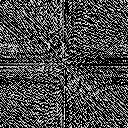
\includegraphics[width=3cm,height=3cm,keepaspectratio]{img/transformed/fft/phase_lena_8.png}}}%
    \qquad
    \qquad
    \subfloat[Lena 8b]{{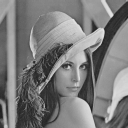
\includegraphics[width=3cm,height=3cm,keepaspectratio]{img/transformed/fft/lena_8.png}}}%
    \qquad
    \qquad
    \caption{Widmo mocy i widmo fazy dla obrazu Lena 8-bitowego.}%
\end{figure} 

\begin{figure}[H]%
    \centering
    \subfloat[Widmo mocy R]{{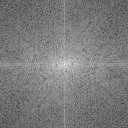
\includegraphics[width=3cm,height=3cm,keepaspectratio]{img/transformed/fft/abs_red_girl_24.png}}}%
    \qquad
    \qquad
    \subfloat[Widmo mocy G]{{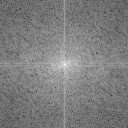
\includegraphics[width=3cm,height=3cm,keepaspectratio]{img/transformed/fft/abs_green_girl_24.png}}}%    
    \qquad
    \qquad
    \subfloat[Widmo mocy B]{{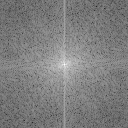
\includegraphics[width=3cm,height=3cm,keepaspectratio]{img/transformed/fft/abs_blue_girl_24.png}}}%    
    \qquad   
    \qquad 
    \subfloat[Widmo fazy R]{{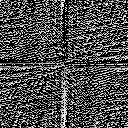
\includegraphics[width=3cm,height=3cm,keepaspectratio]{img/transformed/fft/phase_red_girl_24.png}}}%
    \qquad
    \qquad
    \subfloat[Widmo fazy G]{{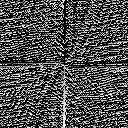
\includegraphics[width=3cm,height=3cm,keepaspectratio]{img/transformed/fft/phase_green_girl_24.png}}}%
    \qquad
    \qquad
    \subfloat[Widmo fazy B]{{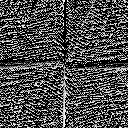
\includegraphics[width=3cm,height=3cm,keepaspectratio]{img/transformed/fft/phase_blue_girl_24.png}}}%
    \qquad
    \qquad
    \subfloat[Girl 24b]{{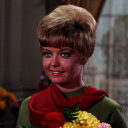
\includegraphics[width=3cm,height=3cm,keepaspectratio]{img/transformed/fft/girl_24.png}}}%
    \qquad
    \caption{Widma mocy i widma fazy dla kanałów RGB obrazu Girl 24-bitowego.}%
\end{figure} 

\subsection{Filtracja}
Sekcja ta prezentuje wyniki zastosowania filtracji dla wybranych obrazów 8-bitowych. Zaprezentowane są próbki oraz widma mocy i fazy przed i po filtracji. 

\subsubsection{Filtr dolnoprzepustowy (górnozaporowy)}
Wyniki zastosowania filtru dolnoprzepustowego na obrazie 8-bitowym Lena zaszumionym szumem jednostajnym 3 są przedstawione poniżej.
\begin{figure}[H]%
    \centering
    \subfloat[Obraz bez filtru]{{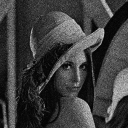
\includegraphics[width=3cm,height=3cm,keepaspectratio]{img/transformed/filters/low-pass/low_pass_lena_uniform_3_before.png}}}%
    \qquad
    \qquad
    \subfloat[Widmo mocy bez filtru]{{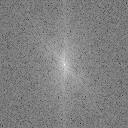
\includegraphics[width=3cm,height=3cm,keepaspectratio]{img/transformed/filters/low-pass/low_pass_abs_before_lena_8.png}}}%    
    \qquad
    \qquad
    \subfloat[Widmo fazy bez filtru]{{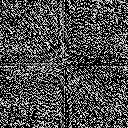
\includegraphics[width=3cm,height=3cm,keepaspectratio]{img/transformed/filters/low-pass/low_pass_phase_before_lena_8.png}}}%    
    \qquad   
    \qquad 
    \subfloat[Obraz z filtrem]{{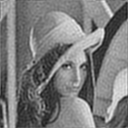
\includegraphics[width=3cm,height=3cm,keepaspectratio]{img/transformed/filters/low-pass/low_pass_lena_uniform_3_after.png}}}%
    \qquad
    \qquad
    \subfloat[Widmo mocy z filtrem]{{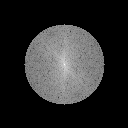
\includegraphics[width=3cm,height=3cm,keepaspectratio]{img/transformed/filters/low-pass/low_pass_abs_after_lena_8.png}}}%
    \qquad
    \qquad
    \subfloat[Widmo fazy z filtrem]{{
\includegraphics[width=3cm,height=3cm,keepaspectratio]{img/transformed/filters/low-pass/low_pass_phase_after_lena_8.png}}}%
    \qquad
    \caption{Zastosowanie filtru dolnoprzepustowego na obrazie Lena 8-bitowym zaszumionym szumem jednostajnym; max=10.}%
\end{figure}  

\subsubsection{Filtr górnoprzepustowy (dolnozaporowy)}
Wyniki zastosowania filtru górnoprzepustowego na obrazie 8-bitowym Pentagon są przedstawione poniżej. 
\begin{figure}[H]%
    \centering
    \subfloat[Obraz bez filtru]{{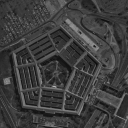
\includegraphics[width=3cm,height=3cm,keepaspectratio]{img/transformed/filters/high-pass/high_pass_pentagon_before.png}}}%
    \qquad
    \qquad
    \subfloat[Widmo mocy bez filtru]{{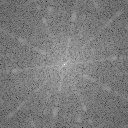
\includegraphics[width=3cm,height=3cm,keepaspectratio]{img/transformed/filters/high-pass/high_pass_abs_before_pentagon_8.png}}}%    
    \qquad
    \qquad
    \subfloat[Widmo fazy bez filtru]{{
\includegraphics[width=3cm,height=3cm,keepaspectratio]{img/transformed/filters/high-pass/high_pass_phase_before_pentagon_8.png}}}%    
    \qquad   
    \qquad 
    \subfloat[Obraz z filtrem]{{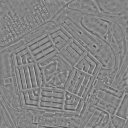
\includegraphics[width=3cm,height=3cm,keepaspectratio]{img/transformed/filters/high-pass/high_pass_pentagon_after.png}}}%
    \qquad
    \qquad
    \subfloat[Widmo mocy z filtrem]{{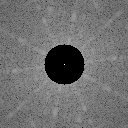
\includegraphics[width=3cm,height=3cm,keepaspectratio]{img/transformed/filters/high-pass/high_pass_abs_after_pentagon_8.png}}}%
    \qquad
    \qquad
    \subfloat[Widmo fazy z filtrem]{{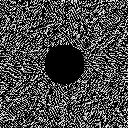
\includegraphics[width=3cm,height=3cm,keepaspectratio]{img/transformed/filters/high-pass/high_pass_phase_after_pentagon_8.png}}}%
    \qquad
    \caption{Zastosowanie filtru górnoprzepustowego na obrazie Pentagon 8-bitowym; min=20.}%
\end{figure}  

\subsubsection{Filtr pasmowoprzepustowy}
Wyniki zastosowania filtru pasmowoprzepustowego na obrazie 8-bitowym Lena są przedstawione poniżej. 
\begin{figure}[H]%
    \centering
    \subfloat[Obraz bez filtru]{{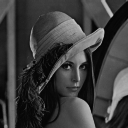
\includegraphics[width=3cm,height=3cm,keepaspectratio]{img/transformed/filters/band-pass/band_pass_lena_before.png}}}%
    \qquad
    \qquad
    \subfloat[Widmo mocy bez filtru]{{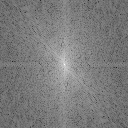
\includegraphics[width=3cm,height=3cm,keepaspectratio]{img/transformed/filters/band-pass/band_pass_abs_before_lena_8.png}}}%    
    \qquad
    \qquad
    \subfloat[Widmo fazy bez filtru]{{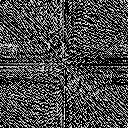
\includegraphics[width=3cm,height=3cm,keepaspectratio]{img/transformed/filters/band-pass/band_pass_phase_before_lena_8.png}}}%    
    \qquad   
    \qquad 
    \subfloat[Obraz z filtem]{{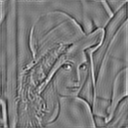
\includegraphics[width=3cm,height=3cm,keepaspectratio]{img/transformed/filters/band-pass/band_pass_lena_after.png}}}%
    \qquad
    \qquad
    \subfloat[Widmo mocy z filtrem]{{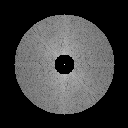
\includegraphics[width=3cm,height=3cm,keepaspectratio]{img/transformed/filters/band-pass/band_pass_abs_after_lena_8.png}}}%
    \qquad
    \qquad
    \subfloat[Widmo fazy z filtrem]{{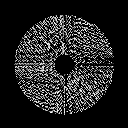
\includegraphics[width=3cm,height=3cm,keepaspectratio]{img/transformed/filters/band-pass/band_pass_phase_after_lena_8.png}}}%
    \qquad
    \caption{Zastosowanie filtru pasmowoprzepustowego na obrazie Lena 8-bitowym; min=10, max=50.}%
\end{figure}  

\subsubsection{Filtr pasmowozaporowy}
Wyniki zastosowania filtru pasmowozaporowego na obrazie 8-bitowym Messer są przedstawione poniżej. 
\begin{figure}[H]%
    \centering
    \subfloat[Obraz bez filtru]{{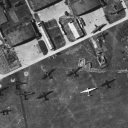
\includegraphics[width=3cm,height=3cm,keepaspectratio]{img/transformed/filters/band-cut/band_cut_messer_before.png}}}%
    \qquad
    \qquad
    \subfloat[Widmo mocy bez filtru]{{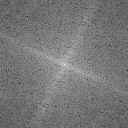
\includegraphics[width=3cm,height=3cm,keepaspectratio]{img/transformed/filters/band-cut/band_cut_abs_before_messer_8.png}}}%    
    \qquad
    \qquad
    \subfloat[Widmo fazy bez filtru]{{
\includegraphics[width=3cm,height=3cm,keepaspectratio]{img/transformed/filters/band-cut/band_cut_phase_before_messer_8.png}}}%    
    \qquad   
    \qquad 
    \subfloat[Obraz z filtem]{{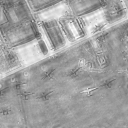
\includegraphics[width=3cm,height=3cm,keepaspectratio]{img/transformed/filters/band-cut/band_cut_messer_after.png}}}%
    \qquad
    \qquad
    \subfloat[Widmo mocy z filtrem]{{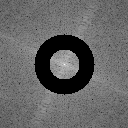
\includegraphics[width=3cm,height=3cm,keepaspectratio]{img/transformed/filters/band-cut/band_cut_abs_after_messer_8.png}}}%
    \qquad
    \qquad
    \subfloat[Widmo fazy z filtrem]{{
\includegraphics[width=3cm,height=3cm,keepaspectratio]{img/transformed/filters/band-cut/band_cut_phase_after_messer_8.png}}}%
    \qquad
    \caption{Zastosowanie filtru pasmowozaporowego na obrazie Messer 8-bitowym; min=15, max=30.}%
\end{figure}  

\subsubsection{Filtr z detekcją krawędzi}
Wyniki zastosowania filtru z detekcją krawędzi na obrazie 8-bitowym Camera są przedstawione poniżej.

\begin{figure}[H]%
    \centering
    \subfloat[Obraz bez filtru]{{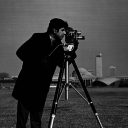
\includegraphics[width=3cm,height=3cm,keepaspectratio]{img/transformed/filters/edge-detection/edge_detection_camera_8_before.png}}}%
    \qquad
    \qquad
    \subfloat[Widmo mocy bez filtru]{{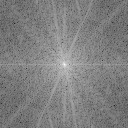
\includegraphics[width=3cm,height=3cm,keepaspectratio]{img/transformed/filters/edge-detection/edge_detection_abs_before_camera_8_mask_1.png}}}%    
    \qquad
    \qquad
    \subfloat[Widmo fazy bez filtru]{{
\includegraphics[width=3cm,height=3cm,keepaspectratio]{img/transformed/filters/edge-detection/edge_detection_phase_before_camera_8_mask_1.png}}}%    
    \qquad   
    \qquad 
    \subfloat[Obraz z filtem]{{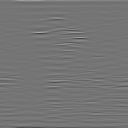
\includegraphics[width=3cm,height=3cm,keepaspectratio]{img/transformed/filters/edge-detection/edge_detection_camera_8_after_mask_1.png}}}%
    \qquad
    \qquad
    \subfloat[Widmo mocy z filtrem]{{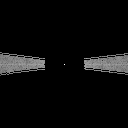
\includegraphics[width=3cm,height=3cm,keepaspectratio]{img/transformed/filters/edge-detection/edge_detection_abs_after_camera_8_mask_1.png}}}%
    \qquad
    \qquad
    \subfloat[Widmo fazy z filtrem]{{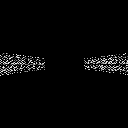
\includegraphics[width=3cm,height=3cm,keepaspectratio]{img/transformed/filters/edge-detection/edge_detection_phase_after_camera_8_mask_1.png}}}%
    \qquad
    \caption{Zastosowanie filtru z detekcją krawędzi i maską 1 na obrazie Camera 8-bitowym; min=20.}%
\end{figure}  

\begin{figure}[H]%
    \centering
    \subfloat[Obraz bez filtru]{{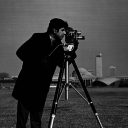
\includegraphics[width=3cm,height=3cm,keepaspectratio]{img/transformed/filters/edge-detection/edge_detection_camera_8_before.png}}}%
    \qquad
    \qquad
    \subfloat[Widmo mocy bez filtru]{{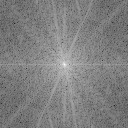
\includegraphics[width=3cm,height=3cm,keepaspectratio]{img/transformed/filters/edge-detection/edge_detection_abs_before_camera_8_mask_2.png}}}%    
    \qquad
    \qquad
    \subfloat[Widmo fazy bez filtru]{{
\includegraphics[width=3cm,height=3cm,keepaspectratio]{img/transformed/filters/edge-detection/edge_detection_phase_before_camera_8_mask_2.png}}}%    
    \qquad   
    \qquad 
    \subfloat[Obraz z filtem]{{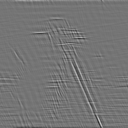
\includegraphics[width=3cm,height=3cm,keepaspectratio]{img/transformed/filters/edge-detection/edge_detection_camera_8_after_mask_2.png}}}%
    \qquad
    \qquad
    \subfloat[Widmo mocy z filtrem]{{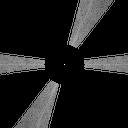
\includegraphics[width=3cm,height=3cm,keepaspectratio]{img/transformed/filters/edge-detection/edge_detection_abs_after_camera_8_mask_2.png}}}%
    \qquad
    \qquad
    \subfloat[Widmo fazy z filtrem]{{
\includegraphics[width=3cm,height=3cm,keepaspectratio]{img/transformed/filters/edge-detection/edge_detection_phase_after_camera_8_mask_2.png}}}%
    \qquad
    \caption{Zastosowanie filtru z detekcją krawędzi i maską 2 na obrazie Camera 8-bitowym; min=20.}%
\end{figure}  

\subsubsection{Filtr modyfikujący fazę widma transformaty Fouriera}
Wyniki zastosowania filtru modyfikującego fazę widma transformaty Foueriera na obrazie 8-bitowym Bird są przedstawione poniżej. 
\begin{figure}[H]%
    \centering
    \subfloat[Obraz bez filtru]{{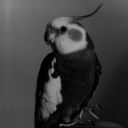
\includegraphics[width=3cm,height=3cm,keepaspectratio]{img/transformed/filters/spectrum-modification/spectrum_modification_bird_before.png}}}%
    \qquad
    \qquad
    \subfloat[Widmo mocy bez filtru]{{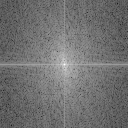
\includegraphics[width=3cm,height=3cm,keepaspectratio]{img/transformed/filters/spectrum-modification/spectrum_modification_abs_before_bird_8.png}}}%    
    \qquad
    \qquad
    \subfloat[Widmo fazy bez filtra]{{\includegraphics[width=3cm,height=3cm,keepaspectratio]{img/transformed/filters/spectrum-modification/spectrum_modification_phase_before_bird_8.png}}}%    
    \qquad   
    \qquad 
    \subfloat[Obraz z filtem]{{\includegraphics[width=3cm,height=3cm,keepaspectratio]{img/transformed/filters/spectrum-modification/spectrum_modification_bird_after.png}}}%
    \qquad
    \qquad
    \subfloat[Widmo mocy z filtrem]{{\includegraphics[width=3cm,height=3cm,keepaspectratio]{img/transformed/filters/spectrum-modification/spectrum_modification_abs_after_bird_8.png}}}%
    \qquad
    \qquad
    \subfloat[Widmo fazy z filtrem]{{\includegraphics[width=3cm,height=3cm,keepaspectratio]{img/transformed/filters/spectrum-modification/spectrum_modification_phase_after_bird_8.png}}}%
    \qquad
    \caption{Zastosowanie filtru modyfikującego fazę widma transformaty Fouriera na obrazie Bird 8-bitowym; k=40, l=200.}%
\end{figure} 

\subsubsection{Okno Hanninga}
Wyniki zastosowania okna Hanninga na obrazie 8-bitowym Lena są przedstawione poniżej.
\begin{figure}[H]%
    \centering
    \subfloat[Obraz po nałożeniu okna Hanninga]{{\includegraphics[width=3cm,height=3cm,keepaspectratio]{img/transformed/hann/hann_window_lena_8.png}}}%
    \qquad
    \qquad
    \subfloat[Widmo mocy]{{\includegraphics[width=3cm,height=3cm,keepaspectratio]{img/transformed/hann/hann_window_abs_lena_8.png}}}%
    \qquad
    \qquad
    \subfloat[Widmo fazy]{{\includegraphics[width=3cm,height=3cm,keepaspectratio]{img/transformed/hann/hann_window_phase_lena_8.png}}}%
    \qquad
    \qquad
    \caption{Zastosowanie okna Hanninga na obrazie 8-bitowym Lena.}%
\end{figure} 

\subsection{Segmentacja}
Sekcja ta prezentuje wyniki wyniki zastosowania segmentacji dla obrazu 24-bitowego Girl. Zaprezentowane są nałożone maski dla różnych parametrów progu i minimalnej ilości pikseli na obszar.

\subsubsection{Metoda rozrostu obszarów}
Wyniki zastosowania metody rozrostu obszarów w celu segmentacji regionów na obrazie 24-bitowym Girl przedstawione są poniżej.
\begin{figure}[H]%
    \centering
    \subfloat[próg=1, minP=200]{{\includegraphics[width=2.5cm,height=2.5cm,keepaspectratio]{img/transformed/segmentation/growing_1_200_girl_24.png}}}%
    \qquad
    \subfloat[próg=5, minP=200]{{\includegraphics[width=2.5cm,height=2.5cm,keepaspectratio]{img/transformed/segmentation/growing_5_200_girl_24.png}}}%    
    \qquad
    \subfloat[próg=10, minP=200]{{\includegraphics[width=2.5cm,height=2.5cm,keepaspectratio]{img/transformed/segmentation/growing_10_200_girl_24.png}}}%    
    \qquad 
    \subfloat[próg=15, minP=200]{{\includegraphics[width=32.5cm,height=2.5cm,keepaspectratio]{img/transformed/segmentation/growing_15_200_girl_24.png}}}%
    \qquad
    \subfloat[próg=1, minP=1000]{{\includegraphics[width=2.5cm,height=2.5cm,keepaspectratio]{img/transformed/segmentation/growing_1_1000_girl_24.png}}}%
    \qquad
    \subfloat[próg=5, minP=1000]{{\includegraphics[width=2.5cm,height=2.5cm,keepaspectratio]{img/transformed/segmentation/growing_5_1000_girl_24.png}}}%    
    \qquad
    \subfloat[próg=10, minP=1000]{{\includegraphics[width=2.5cm,height=2.5cm,keepaspectratio]{img/transformed/segmentation/growing_10_1000_girl_24.png}}}%    
    \qquad 
    \subfloat[próg=15, minP=1000]{{\includegraphics[width=32.5cm,height=2.5cm,keepaspectratio]{img/transformed/segmentation/growing_15_1000_girl_24.png}}}%
    \qquad
    \caption{Zastosowanie metody rozrostu obszarów w celu segmentacji regionów na obrazie 24-bitowym Girl.}%
\end{figure} 

\subsubsection{Metoda podziału obszarów}
Wyniki zastosowania metody podziału obszarów w celu segmentacji regionów na obrazie 24-bitowym Girl przedstawione są poniżej.
\begin{figure}[H]%
    \centering
    \subfloat[próg=1, minP=200]{{\includegraphics[width=2.5cm,height=2.5cm,keepaspectratio]{img/transformed/segmentation/split_merge_1_200_girl_24.png}}}%
    \qquad
    \subfloat[próg=5, minP=200]{{\includegraphics[width=2.5cm,height=2.5cm,keepaspectratio]{img/transformed/segmentation/split_merge_5_200_girl_24.png}}}%    
    \qquad
    \subfloat[próg=10, minP=200]{{\includegraphics[width=2.5cm,height=2.5cm,keepaspectratio]{img/transformed/segmentation/split_merge_10_200_girl_24.png}}}%    
    \qquad 
    \subfloat[próg=15, minP=200]{{\includegraphics[width=32.5cm,height=2.5cm,keepaspectratio]{img/transformed/segmentation/split_merge_15_200_girl_24.png}}}%
    \qquad
    \subfloat[próg=1, minP=1000]{{\includegraphics[width=2.5cm,height=2.5cm,keepaspectratio]{img/transformed/segmentation/split_merge_1_1000_girl_24.png}}}%
    \qquad
    \subfloat[próg=5, minP=1000]{{\includegraphics[width=2.5cm,height=2.5cm,keepaspectratio]{img/transformed/segmentation/split_merge_5_1000_girl_24.png}}}%    
    \qquad
    \subfloat[próg=10, minP=1000]{{\includegraphics[width=2.5cm,height=2.5cm,keepaspectratio]{img/transformed/segmentation/split_merge_10_1000_girl_24.png}}}%    
    \qquad 
    \subfloat[próg=15, minP=1000]{{\includegraphics[width=32.5cm,height=2.5cm,keepaspectratio]{img/transformed/segmentation/split_merge_15_1000_girl_24.png}}}%
    \qquad
    \caption{Zastosowanie metody podziału obszarów w celu segmentacji regionów na obrazie 24-bitowym Girl.}%
\end{figure} 

\section{Dyskusja i wnioski}
Poniższa sekcja prezentuje interpretację uzyskanych wyników oraz wnioski. Opisano również napotkane problemy oraz możliwe sposoby ich rozwiązania.

\subsection{Filtracja}
Nałożenie filtru dolnoprzepustowego powoduje usuwanie wysokich częstotliwości z obrazu. Może być on zatem zastosowany do odszumiania próbek (rys. 4). Im większa wartość współczynnika d$_{\text{min}}$, tym rezultat jest bardziej rozmazany.\\
\\
\indent
Filtr górnoprzepustowy może być wykorzystywany do wyszukiwania krawędzi w obrazie, ponieważ usuwa elementy o niskiej częstotliwości (rys. 5). Ważnym elementem filtru jest tzw. \textit{DC component}, który jest częstotliwością zerową i nie powinien być naruszany w wyniku modyfikacji.\\
\\
\indent
Filtr pasmowoprzepustowy usuwa z obrazu zarówno częstotliwości wysokie, jak i niskie. Pozostawia jedynie wybrany przez użytkownika zakres (rys. 6).\\
\\
\indent
Filtr pasmowozaporowy jest używany do usuwania wybranego zakresu częstotliwości, pozostawiając te najwyższe i najniższe (rys. 7).\\
\\
\indent
Filtr z detekcją krawędzi, będący modyfikacją filtru górnoprzepustowego, poprawnie wyszukał krawędzie we wskazanych przez maski kierunkach (rys. 8 i rys. 9). Zwłaszcza statyw kamery jest doskonale widoczny (rys. 9a).\\
\\
\indent
Nałożenie filtru modyfikującego fazę widma transformaty Fouriera powoduje przesunięcie pionowe i poziome obrazu (rys. 10). Wartości dodanie przemieszczają rezultat w dół i w prawo, natomiast ujemne - w górę i w lewo.\\
\\
\indent
Nałożenie okna Hanninga powoduje stopniowe wyciemnianie obrazu wynikowego na jego krańcach (rys. 11a). Dzięki temu wszelkie błędy wynikające z dyskretnego charaketeru sygnału wejściowego są niewidoczne. Wyraźnie widać różnicę w widmie mocy i fazy dla obrazu z nałożonym oknem (rys. 11b i 11c) w porównaniu do zwykłego przekształcenia (rys. 2a i 2b).

\subsection{Segmentacja}
Zastosowanie metody rozrostu obszarów w procesie segmentacji przyniosło bardzo dobre rezultaty. Na początku badania wybrano 64 ziarna, równomiernie rozłożone na obrazie. Znalezione regiony bardzo dobrze oddawały faktyczne skupiska pikseli o podobnych kolorych (rys. 12c, rys. 12d).\\
\\
\indent
Metoda podziału obszarów również dobrze spełniła swoje zadanie. Wyniki okazały się jednak zauważalnie gorsze od tych uzyskanych w wyniku analizy metody rozrostu. Prawdopodobnie było to spowodowane metodą łączenia obszarów, która była inicjalowana po całym procesie podziału, zamiast po każdorazowym tworzeniu nowych regionów. 

\begin{thebibliography}{1}
\bibitem{instruction_pol}\text{$http://ftims.edu.p.lodz.pl/pluginfile.php/19300/mod\_resource/content/3/$}\\
\text{$Zadanie2.pdf, 2015$}
\bibitem{instruction_pol}\text{$http://ftims.edu.p.lodz.pl/pluginfile.php/19301/mod\_resource/content/0/$}\\
\text{$dft.pdf, 2015$}
\bibitem{instruction_pol}\text{$https://github.com/alisowsk/image-and-sound-processing/blob/master/$}\\
\text{$sprawozdanie/sprawozdanie.pdf, 2015$}
\bibitem{instruction_ang}\text{$http://ics.p.lodz.pl/~tomczyk/available/po\_en/second.html, 2015$}
\bibitem{instruction_latex}\text{$https://en.wikibooks.org/wiki/LaTeX/Mathematics, 2015$}
\bibitem{doc_linear_fitering}\text{$http://lodev.org/cgtutor/fourier.html, 2015$}
\bibitem{doc_linear_fitering}\text{$http://www.doc.ic.ac.uk/~dfg/vision/v02.html, 2015$}
\bibitem{doc_linear_fitering}\text{$http://fourier.eng.hmc.edu/e101/lectures/Image\_Processing/node6.html, 2015$}
\bibitem{doc_linear_fitering}\text{$http://users.ecs.soton.ac.uk/msn/book/new\_demo/fourier/, 2015$}
\bibitem{doc_linear_fitering}\text{$https://pl.wikipedia.org/wiki/Algorytm\_Cooleya-Tukeya, 2015$}
\bibitem{doc_linear_fitering}\text{$http://librow.com/articles/article-10, 2015$}
\bibitem{doc_linear_fitering}\text{$https://www.cs.cf.ac.uk/Dave/Vision\_lecture/node34.html, 2015$}
\end{thebibliography}

\end{document}
